\label{3.5 C5S Answer Key}
\subsection{Answer Key}
\tiny
\renewcommand{\insertclass}{- Class 5}
\renewcommand{\insertsubject}{ - Science}

\begin{frame}[shrink=0.1,label=QPC5QC5S01 - DT - Q3]{Q5 [1. Living organisms and their environment*]}
\vspace{-0.2cm}

\mcqtextbottomOneFour{
  questionnumber={5}, 
  questionTag={C5S01 – DT – Q3}, 
  questiontext={Which of the following dog’s senses is very useful for humans?},
  optionA={Hearing},
  optionB={Smell},
  optionC={Taste},
  optionD={Touch},
  correctoption={B},
}


\begin{minipage}{\linewidth}
\hspace{1cm}
\centering
\tiny
\renewcommand{\arraystretch}{1.25}
\begin{tabular}{|M{1.2cm}|M{0.8cm}|M{0.8cm}|M{0.8cm}|M{0.8cm}|M{0.8cm}|}
\hline
Option & A (\ding{55}) & \cellcolor{cellgreen} B (\ding{51}) & C (\ding{55}) & D (\ding{55}) & E \\ 
\hline
5 A & \highno{0\%} & \highgreen{94\%} & \highno{0\%} & \highno{6\%} & \highno{0\%} \\ 
 \hline 
5 B & \highno{21\%} & \highno{71\%} & \highno{7\%} & \highno{0\%} & \highno{0\%} \\ \hline
\end{tabular}
\end{minipage}

\end{frame}
% \input{4. PPT/My Answer/Science/C5/117_C5S - Q5}


\begin{frame}[shrink=0.1,label=QPC5QC5S01 - DT - Q7]{Q11 [1. Living organisms and their environment*]}
\vspace{-0.2cm}
\mcqtextbottomOneFour{
  questionnumber={11}, 
  questionTag={C5S01 – DT – Q7}, 
  questiontext={Which of these animals can live both in water and on land?},
  optionA={\adjustbox{scale=\scalefactor}{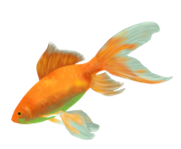
\includegraphics[width=3cm,height=2.5cm]{C5BZ – DT – Q3i.png}}},
  optionB={\adjustbox{scale=\scalefactor}{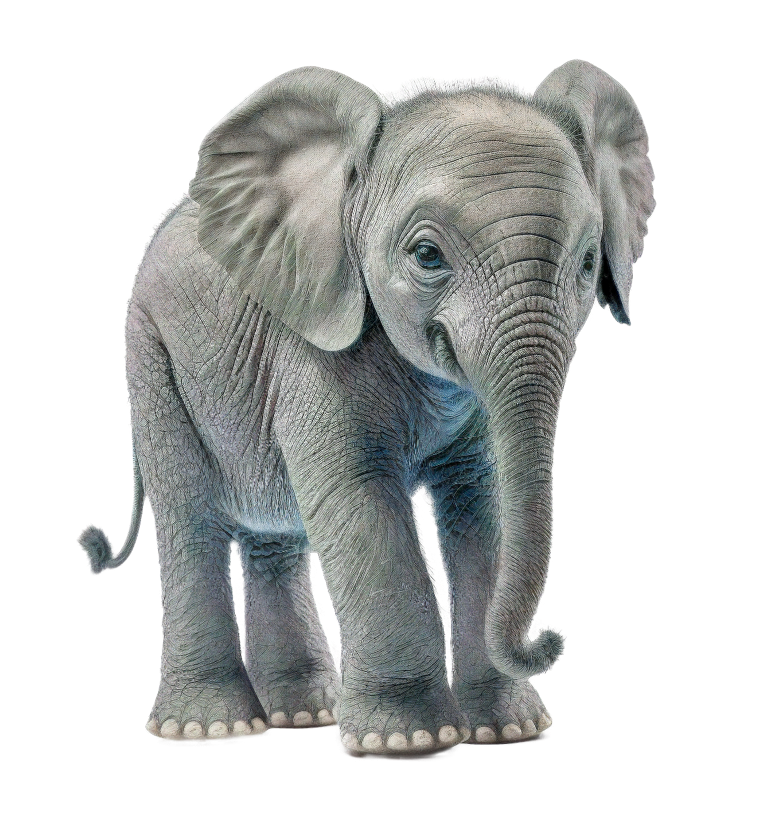
\includegraphics[width=3cm,height=2.5cm]{C5BZ – DT – Q3ii.png}}},
  optionC={\adjustbox{scale=\scalefactor}{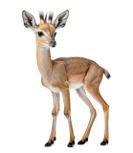
\includegraphics[width=3cm,height=2.5cm]{C5BZ – DT – Q3iii.png}}},
  optionD={\adjustbox{scale=\scalefactor}{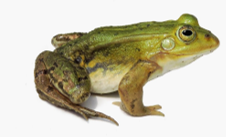
\includegraphics[width=3cm,height=2.5cm]{C5BZ – DT – Q3iv.png}}},
  correctoption={D},
}

\begin{minipage}{\linewidth}
\hspace{1cm}
\centering
\tiny
\renewcommand{\arraystretch}{1.25}
\begin{tabular}{|M{1.2cm}|M{0.8cm}|M{0.8cm}|M{0.8cm}|M{0.8cm}|M{0.8cm}|}
\hline
Option & A (\ding{55}) & B (\ding{55}) & C (\ding{55}) & \cellcolor{cellgreen} D (\ding{51}) & E \\ 
\hline
5 A & \highno{6\%} & \highno{0\%} & \highno{6\%} & \highgreen{82\%} & \highno{6\%} \\ 
 \hline 
5 B & \highno{0\%} & \highno{7\%} & \highno{0\%} & \highgreen{93\%} & \highno{0\%} \\ \hline
\end{tabular}
\end{minipage}

\end{frame}
% \input{4. PPT/My Answer/Science/C5/117_C5S - Q11}


\begin{frame}[shrink=0.1,label=QPC5QC5S01 - DT - Q2]{Q33 [1. Living organisms and their environment*]}
\vspace{-0.2cm}

\mcqtextbottomOneFour{
  questionnumber={33}, 
  questionTag={C5S01 – DT – Q2}, 
  questiontext={Which part of the plant absorbs water and nutrients from soil? },
  optionA={Flower},
  optionB={Stem},
  optionC={Leaves},
  optionD={Root},
  correctoption={D},
}


\begin{minipage}{\linewidth}
\hspace{1cm}
\centering
\tiny
\renewcommand{\arraystretch}{1.25}
\begin{tabular}{|M{1.2cm}|M{0.8cm}|M{0.8cm}|M{0.8cm}|M{0.8cm}|M{0.8cm}|}
\hline
Option & A (\ding{55}) & B (\ding{55}) & C (\ding{55}) & \cellcolor{cellgreen} D (\ding{51}) & E \\ 
\hline
5 A & \highno{0\%} & \highno{6\%} & \highno{0\%} & \highgreen{94\%} & \highno{0\%} \\ 
 \hline 
5 B & \highno{0\%} & \highno{0\%} & \highno{0\%} & \highgreen{100\%} & \highno{0\%} \\ \hline
\end{tabular}
\end{minipage}

\end{frame}
% \input{4. PPT/My Answer/Science/C5/117_C5S - Q33}


\begin{frame}[shrink=0.1,label=QPC5QC5S01 - DT - Q8]{Q34 [1. Living organisms and their environment*]}
\vspace{-0.2cm}
\mcqtextbottomOneFour{
  questionnumber={34}, 
  questionTag={C5S01 – DT – Q8}, 
  questiontext={Which body part helps a bird to fly?},
  optionA={Legs},
  optionB={Eyes},
  optionC={Wings},
  optionD={Tail},
  correctoption={C},
}

\begin{minipage}{\linewidth}
\hspace{1cm}
\centering
\tiny
\renewcommand{\arraystretch}{1.25}
\begin{tabular}{|M{1.2cm}|M{0.8cm}|M{0.8cm}|M{0.8cm}|M{0.8cm}|M{0.8cm}|}
\hline
Option & A (\ding{55}) & B (\ding{55}) & \cellcolor{cellgreen} C (\ding{51}) & D (\ding{55}) & E \\ 
\hline
5 A & \highno{6\%} & \highno{0\%} & \highgreen{82\%} & \highno{12\%} & \highno{0\%} \\ 
 \hline 
5 B & \highno{0\%} & \highno{7\%} & \highgreen{79\%} & \highno{14\%} & \highno{0\%} \\ \hline
\end{tabular}
\end{minipage}

\end{frame}
% \input{4. PPT/My Answer/Science/C5/117_C5S - Q34}


\begin{frame}[shrink=0.1,label=QPC5QC5S01 - DT - Q1]{Q38 [1. Living organisms and their environment*]}
\vspace{-0.2cm}
\mcqtextbottomOneFour{
  questionnumber={38}, 
  questionTag={C5S01 – DT – Q1}, 
  questiontext={Identify the living object from the following images.},
  optionA={\adjustbox{scale=\scalefactor}{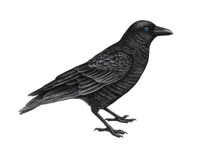
\includegraphics[width=3cm,height=2.5cm]{C5S01 – DT – Q1i.png}}},
  optionB={\adjustbox{scale=\scalefactor}{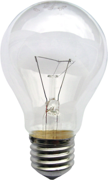
\includegraphics[width=1.5cm,height=2.5cm]{C5S01 – DT – Q1ii.png}}},
  optionC={\adjustbox{scale=\scalefactor}{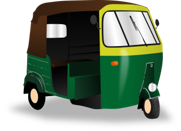
\includegraphics[width=3.5cm,height=2.5cm]{C5S01 – DT – Q1iii.png}}},
  optionD={\adjustbox{scale=\scalefactor}{
\includegraphics[width=2.5cm,height=2.5cm]{C5S01 – DT – Q1iv.png}}},
  correctoption={A},
}

\begin{minipage}{\linewidth}
\hspace{1cm}
\centering
\tiny
\renewcommand{\arraystretch}{1.25}
\begin{tabular}{|M{1.2cm}|M{0.8cm}|M{0.8cm}|M{0.8cm}|M{0.8cm}|M{0.8cm}|}
\hline
Option & \cellcolor{cellgreen} A (\ding{51}) & B (\ding{55}) & C (\ding{55}) & D (\ding{55}) & E \\ 
\hline
5 A & \highgreen{100\%} & \highno{0\%} & \highno{0\%} & \highno{0\%} & \highno{0\%} \\ 
 \hline 
5 B & \highgreen{100\%} & \highno{0\%} & \highno{0\%} & \highno{0\%} & \highno{0\%} \\ \hline
\end{tabular}
\end{minipage}

\end{frame}
% \input{4. PPT/My Answer/Science/C5/117_C5S - Q38}


\begin{frame}[shrink=0.1,label=QPC5QC5S02 - DT - Q5]{Q10\small [2. Basic needs of living organisms (food, water, air, shelter)*]}
\vspace{-0.2cm}
\mcqtextbottomFourOne{
  questionnumber={10}, 
  questionTag={C5S02 – DT – Q5}, 
  questiontext={Why do living organisms need shelter?},
  optionA={To store water.},
  optionB={To prepare food.},
  optionC={To protect from extreme climate conditions.},
  optionD={To produce energy for survival.},
  correctoption={C},
}

\begin{minipage}{\linewidth}
\hspace{1cm}
\centering
\tiny
\renewcommand{\arraystretch}{1.25}
\begin{tabular}{|M{1.2cm}|M{0.8cm}|M{0.8cm}|M{0.8cm}|M{0.8cm}|M{0.8cm}|}
\hline
Option & A (\ding{55}) & B (\ding{55}) & \cellcolor{cellgreen} C (\ding{51}) & D (\ding{55}) & E \\ 
\hline
5 A & \highno{0\%} & \highno{24\%} & \highno{59\%} & \highno{12\%} & \highno{6\%} \\ 
 \hline 
5 B & \highno{29\%} & \highno{7\%} & \highno{50\%} & \highno{7\%} & \highno{7\%} \\ \hline
\end{tabular}
\end{minipage}

\end{frame}
% \input{4. PPT/My Answer/Science/C5/117_C5S - Q10}


\begin{frame}[shrink=0.1,label=QPC5QC5S02 - DT - Q8]{Q14\small [2. Basic needs of living organisms (food, water, air, shelter)*]}
\vspace{-0.2cm}
\mcqtextbottomOneFour{
  questionnumber={14}, 
  questionTag={C5S02 – DT – Q8}, 
  questiontext={Which of these comes from a cow?},
  optionA={Wool},
  optionB={Milk},
  optionC={Eggs},
  optionD={Silk},
  correctoption={B},
}

\begin{minipage}{\linewidth}
\hspace{1cm}
\centering
\tiny
\renewcommand{\arraystretch}{1.25}
\begin{tabular}{|M{1.2cm}|M{0.8cm}|M{0.8cm}|M{0.8cm}|M{0.8cm}|M{0.8cm}|}
\hline
Option & A (\ding{55}) & \cellcolor{cellgreen} B (\ding{51}) & C (\ding{55}) & D (\ding{55}) & E \\ 
\hline
5 A & \highno{6\%} & \highgreen{88\%} & \highno{6\%} & \highno{0\%} & \highno{0\%} \\ 
 \hline 
5 B & \highno{0\%} & \highgreen{100\%} & \highno{0\%} & \highno{0\%} & \highno{0\%} \\ \hline
\end{tabular}
\end{minipage}

\end{frame}
% \input{4. PPT/My Answer/Science/C5/117_C5S - Q14}


\begin{frame}[shrink=0.1,label=QPC5QC5S02 - DT - Q11]{Q17\small [2. Basic needs of living organisms (food, water, air, shelter)*]}
\vspace{-0.2cm}
\mcqtextbottomTwoTwo{
  questionnumber={17}, 
  questionTag={C5S02 – DT – Q11}, 
  questiontext={Where can we find air?},
  optionA={Only in trees},
  optionB={Only in sky},
  optionC={Everywhere around us},
  optionD={Only in water},
  correctoption={C},
}

\begin{minipage}{\linewidth}
\hspace{1cm}
\centering
\tiny
\renewcommand{\arraystretch}{1.25}
\begin{tabular}{|M{1.2cm}|M{0.8cm}|M{0.8cm}|M{0.8cm}|M{0.8cm}|M{0.8cm}|}
\hline
Option & A (\ding{55}) & B (\ding{55}) & \cellcolor{cellgreen} C (\ding{51}) & D (\ding{55}) & E \\ 
\hline
5 A & \highno{0\%} & \highno{12\%} & \highgreen{88\%} & \highno{0\%} & \highno{0\%} \\ 
 \hline 
5 B & \highno{29\%} & \highno{7\%} & \highno{64\%} & \highno{0\%} & \highno{0\%} \\ \hline
\end{tabular}
\end{minipage}

\end{frame}
% \input{4. PPT/My Answer/Science/C5/117_C5S - Q17}


\begin{frame}[shrink=0.1,label=QPC5QC5S02 - DT - Q2]{Q21\small [2. Basic needs of living organisms (food, water, air, shelter)*]}
\vspace{-0.2cm}
\mcqtextbottomOneFour{
  questionnumber={21}, 
  questionTag={C5S02 – DT – Q2}, 
  questiontext={The taste of an unripe mango is \rule{80pt}{0.5pt}.},
  optionA={Sour},
  optionB={Sweet},
  optionC={Bitter},
  optionD={Salt},
  correctoption={A},
}

\begin{minipage}{\linewidth}
\hspace{1cm}
\centering
\tiny
\renewcommand{\arraystretch}{1.25}
\begin{tabular}{|M{1.2cm}|M{0.8cm}|M{0.8cm}|M{0.8cm}|M{0.8cm}|M{0.8cm}|}
\hline
Option & \cellcolor{cellgreen} A (\ding{51}) & B (\ding{55}) & C (\ding{55}) & D (\ding{55}) & E \\ 
\hline
5 A & \highno{59\%} & \highno{18\%} & \highno{24\%} & \highno{0\%} & \highno{0\%} \\ 
 \hline 
5 B & \highno{43\%} & \highno{36\%} & \highno{14\%} & \highno{7\%} & \highno{0\%} \\ \hline
\end{tabular}
\end{minipage}

\end{frame}
% \input{4. PPT/My Answer/Science/C5/117_C5S - Q21}


\begin{frame}[shrink=0.1,label=QPC5QC5S02 - DT - Q3]{Q24\small [2. Basic needs of living organisms (food, water, air, shelter)*]}
\vspace{-0.2cm}
\mcqtextbottomFourOne{
  questionnumber={24}, 
  questionTag={C5S02 – DT – Q3}, 
  questiontext={What is the purpose of the expiry date in packed food?},
  optionA={To identify the taste of the food using QR code.},
  optionB={To provide information on when the food was manufactured.},
  optionC={To ensure food is safe to eat.},
  optionD={To indicate the ingredients used in the food.},
  correctoption={C},
}

\begin{minipage}{\linewidth}
\hspace{1cm}
\centering
\tiny
\renewcommand{\arraystretch}{1.25}
\begin{tabular}{|M{1.2cm}|M{0.8cm}|M{0.8cm}|M{0.8cm}|M{0.8cm}|M{0.8cm}|}
\hline
Option & A (\ding{55}) & B (\ding{55}) & \cellcolor{cellgreen} C (\ding{51}) & D (\ding{55}) & E \\ 
\hline
5 A & \highno{12\%} & \highno{24\%} & \highno{53\%} & \highno{12\%} & \highno{0\%} \\ 
 \hline 
5 B & \highno{7\%} & \highno{43\%} & \highno{50\%} & \highno{0\%} & \highno{0\%} \\ \hline
\end{tabular}
\end{minipage}

\end{frame}
% \input{4. PPT/My Answer/Science/C5/117_C5S - Q24}


\begin{frame}[shrink=0.1,label=QPC5QC5S02 - DT - Q1]{Q28\small [2. Basic needs of living organisms (food, water, air, shelter)*]}
\vspace{-0.2cm}
\mcqtextbottomOneFour{
  questionnumber={28}, 
  questionTag={C5S02 – DT – Q1}, 
  questiontext={Find the healthiest food.},
  optionA={Fruits },
  optionB={French fries },
  optionC={Burger },
  optionD={Pizza },
  correctoption={A},
}

\begin{minipage}{\linewidth}
\hspace{1cm}
\centering
\tiny
\renewcommand{\arraystretch}{1.25}
\begin{tabular}{|M{1.2cm}|M{0.8cm}|M{0.8cm}|M{0.8cm}|M{0.8cm}|M{0.8cm}|}
\hline
Option & \cellcolor{cellgreen} A (\ding{51}) & B (\ding{55}) & C (\ding{55}) & D (\ding{55}) & E \\ 
\hline
5 A & \highgreen{94\%} & \highno{0\%} & \highno{6\%} & \highno{0\%} & \highno{0\%} \\ 
 \hline 
5 B & \highgreen{93\%} & \highno{0\%} & \highno{7\%} & \highno{0\%} & \highno{0\%} \\ \hline
\end{tabular}
\end{minipage}

\end{frame}
% \input{4. PPT/My Answer/Science/C5/117_C5S - Q28}


\begin{frame}[shrink=0.1,label=QPC5QC5S02 - DT - Q9]{Q29\small [2. Basic needs of living organisms (food, water, air, shelter)*]}
\vspace{-0.2cm}
\mcqtextbottomTwoTwo{
  questionnumber={29}, 
  questionTag={C5S02 – DT – Q9}, 
  questiontext={What should we do to save water?},
  optionA={Leave the tap running while washing dishes.},
  optionB={Watering the plants during rain.},
  optionC={Take long showers every day.},
  optionD={Turn off the taps when not in use},
  correctoption={D},
}

\begin{minipage}{\linewidth}
\hspace{1cm}
\centering
\tiny
\renewcommand{\arraystretch}{1.25}
\begin{tabular}{|M{1.2cm}|M{0.8cm}|M{0.8cm}|M{0.8cm}|M{0.8cm}|M{0.8cm}|}
\hline
Option & A (\ding{55}) & B (\ding{55}) & C (\ding{55}) & \cellcolor{cellgreen} D (\ding{51}) & E \\ 
\hline
5 A & \highno{12\%} & \highno{6\%} & \highno{0\%} & \highgreen{82\%} & \highno{0\%} \\ 
 \hline 
5 B & \highno{0\%} & \highno{0\%} & \highno{0\%} & \highgreen{100\%} & \highno{0\%} \\ \hline
\end{tabular}
\end{minipage}

\end{frame}
% \input{4. PPT/My Answer/Science/C5/117_C5S - Q29}


\begin{frame}[shrink=0.1,label=QPC5QC5S02 - DT - Q6]{Q32\small [2. Basic needs of living organisms (food, water, air, shelter)*]}
\vspace{-0.2cm}
\mcqtextbottomTwoTwo{
  questionnumber={32}, 
  questionTag={C5S02 – DT – Q6}, 
  questiontext={Why do we separate stones from rice before cooking? },
  optionA={To make food taste better.},
  optionB={To change the color of rice},
  optionC={To play with the picked stone from the rice},
  optionD={To remove harmful or unwanted materials },
  correctoption={D},
}

\begin{minipage}{\linewidth}
\hspace{1cm}
\centering
\tiny
\renewcommand{\arraystretch}{1.25}
\begin{tabular}{|M{1.2cm}|M{0.8cm}|M{0.8cm}|M{0.8cm}|M{0.8cm}|M{0.8cm}|}
\hline
Option & A (\ding{55}) & B (\ding{55}) & C (\ding{55}) & \cellcolor{cellgreen} D (\ding{51}) & E \\ 
\hline
5 A & \highno{12\%} & \highno{0\%} & \highno{12\%} & \highgreen{76\%} & \highno{0\%} \\ 
 \hline 
5 B & \highno{7\%} & \highno{0\%} & \highno{7\%} & \highgreen{86\%} & \highno{0\%} \\ \hline
\end{tabular}
\end{minipage}

\end{frame}
% \input{4. PPT/My Answer/Science/C5/117_C5S - Q32}


\begin{frame}[shrink=0.1,label=QPC5QC5S02 - DT - Q10]{Q37\small [2. Basic needs of living organisms (food, water, air, shelter)*]}
\vspace{-0.2cm}
\mcqtextbottomOneFour{
  questionnumber={37}, 
  questionTag={C5S02 – DT – Q10}, 
  questiontext={Which of these is a natural source of water?},
  optionA={Rain water},
  optionB={Purified water},
  optionC={Tap water},
  optionD={Boiled water},
  correctoption={A},
}

\begin{minipage}{\linewidth}
\hspace{1cm}
\centering
\tiny
\renewcommand{\arraystretch}{1.25}
\begin{tabular}{|M{1.2cm}|M{0.8cm}|M{0.8cm}|M{0.8cm}|M{0.8cm}|M{0.8cm}|}
\hline
Option & \cellcolor{cellgreen} A (\ding{51}) & B (\ding{55}) & C (\ding{55}) & D (\ding{55}) & E \\ 
\hline
5 A & \highgreen{76\%} & \highno{18\%} & \highno{0\%} & \highno{6\%} & \highno{0\%} \\ 
 \hline 
5 B & \highno{71\%} & \highno{7\%} & \highno{7\%} & \highno{14\%} & \highno{0\%} \\ \hline
\end{tabular}
\end{minipage}

\end{frame}
% \input{4. PPT/My Answer/Science/C5/117_C5S - Q37}


\begin{frame}[shrink=0.1,label=QPC5QC5S02 - DT - Q7]{Q39\small [2. Basic needs of living organisms (food, water, air, shelter)*]}
\vspace{-0.2cm}
\mcqtextbottomTwoTwo{
  questionnumber={39}, 
  questionTag={C5S02 – DT – Q7}, 
  questiontext={Why do we feel tired if we skip breakfast?},
  optionA={Our stomach gets too full.},
  optionB={Our body lacks energy.},
  optionC={Feel sleepy because of no rest},
  optionD={Due to the over-workout},
  correctoption={B},
}

\begin{minipage}{\linewidth}
\hspace{1cm}
\centering
\tiny
\renewcommand{\arraystretch}{1.25}
\begin{tabular}{|M{1.2cm}|M{0.8cm}|M{0.8cm}|M{0.8cm}|M{0.8cm}|M{0.8cm}|}
\hline
Option & A (\ding{55}) & \cellcolor{cellgreen} B (\ding{51}) & C (\ding{55}) & D (\ding{55}) & E \\ 
\hline
5 A & \highno{6\%} & \highgreen{76\%} & \highno{6\%} & \highno{12\%} & \highno{0\%} \\ 
 \hline 
5 B & \highno{14\%} & \highno{50\%} & \highno{14\%} & \highno{21\%} & \highno{0\%} \\ \hline
\end{tabular}
\end{minipage}

\end{frame}
% \input{4. PPT/My Answer/Science/C5/117_C5S - Q39}


\begin{frame}[shrink=0.1,label=QPC5QC5S03 - DT - Q3]{Q19 [3. Human body and health*]}
\vspace{-0.2cm}
\mcqtextbottomFourOne{
  questionnumber={19}, 
  questionTag={C5S03 – DT – Q3}, 
  questiontext={Why should we eat the food slowly and chew them properly?},
  optionA={To identify the taste of the food.},
  optionB={It makes your teeth stronger.},
  optionC={This helps in the proper digestion of food.},
  optionD={To avoid eating too much of food.},
  correctoption={C},
}

\begin{minipage}{\linewidth}
\hspace{1cm}
\centering
\tiny
\renewcommand{\arraystretch}{1.25}
\begin{tabular}{|M{1.2cm}|M{0.8cm}|M{0.8cm}|M{0.8cm}|M{0.8cm}|M{0.8cm}|}
\hline
Option & A (\ding{55}) & B (\ding{55}) & \cellcolor{cellgreen} C (\ding{51}) & D (\ding{55}) & E \\ 
\hline
5 A & \highno{6\%} & \highno{0\%} & \highgreen{88\%} & \highno{6\%} & \highno{0\%} \\ 
 \hline 
5 B & \highno{7\%} & \highno{0\%} & \highgreen{86\%} & \highno{7\%} & \highno{0\%} \\ \hline
\end{tabular}
\end{minipage}

\end{frame}
% \input{4. PPT/My Answer/Science/C5/117_C5S - Q19}


\begin{frame}[shrink=0.1,label=QPC5QC5S03 - DT - Q4]{Q26 [3. Human body and health*]}
\vspace{-0.2cm}
\mcqtextbottomOneFour{
  questionnumber={26}, 
  questionTag={C5S03 – DT – Q4}, 
  questiontext={Which among the following diseases are not caused due to mosquitoes?},
  optionA={Malaria},
  optionB={Chikungunya},
  optionC={Chicken pox},
  optionD={Dengue},
  correctoption={C},
}

\begin{minipage}{\linewidth}
\hspace{1cm}
\centering
\tiny
\renewcommand{\arraystretch}{1.25}
\begin{tabular}{|M{1.2cm}|M{0.8cm}|M{0.8cm}|M{0.8cm}|M{0.8cm}|M{0.8cm}|}
\hline
Option & A (\ding{55}) & B (\ding{55}) & \cellcolor{cellgreen} C (\ding{51}) & D (\ding{55}) & E \\ 
\hline
5 A & \highno{6\%} & \highno{24\%} & \highno{65\%} & \highno{6\%} & \highno{0\%} \\ 
 \hline 
5 B & \highno{7\%} & \highno{21\%} & \highno{64\%} & \highno{7\%} & \highno{0\%} \\ \hline
\end{tabular}
\end{minipage}

\end{frame}
% \input{4. PPT/My Answer/Science/C5/117_C5S - Q26}


\begin{frame}[shrink=0.1,label=QPC5QC5S03 - DT - Q1]{Q40 [3. Human body and health*]}
\vspace{-0.2cm}
\mcqtextbottomTwoTwo{
  questionnumber={40}, 
  questionTag={C5S03 – DT – Q1}, 
  questiontext={Find the incorrect pair based on parts of the human body and its function.},
  optionA={Tongue –  Taste},
  optionB={Ear - Chew},
  optionC={Nose - Smell},
  optionD={Eyes - Vision},
  correctoption={B},
}

\begin{minipage}{\linewidth}
\hspace{1cm}
\centering
\tiny
\renewcommand{\arraystretch}{1.25}
\begin{tabular}{|M{1.2cm}|M{0.8cm}|M{0.8cm}|M{0.8cm}|M{0.8cm}|M{0.8cm}|}
\hline
Option & A (\ding{55}) & \cellcolor{cellgreen} B (\ding{51}) & C (\ding{55}) & D (\ding{55}) & E \\ 
\hline
5 A & \highno{0\%} & \highgreen{82\%} & \highno{6\%} & \highno{6\%} & \highno{6\%} \\ 
 \hline 
5 B & \highno{7\%} & \highno{50\%} & \highno{21\%} & \highno{21\%} & \highno{0\%} \\ \hline
\end{tabular}
\end{minipage}

\end{frame}
% \input{4. PPT/My Answer/Science/C5/117_C5S - Q40}


\begin{frame}[shrink=0.1,label=QPC5QC5S04 - DT - Q1]{Q9 [4. Our Earth*]}
\vspace{-0.2cm}
\mcqtextbottomTwoTwo{
  questionnumber={9}, 
  questionTag={C5S04 – DT – Q1}, 
  questiontext={Find the correct pair.},
  optionA={1 week – 6 days},
  optionB={1 year – 365 days},
  optionC={1 month – 25 days},
  optionD={1 decade – 1 year},
  correctoption={B},
}

\begin{minipage}{\linewidth}
\hspace{1cm}
\centering
\tiny
\renewcommand{\arraystretch}{1.25}
\begin{tabular}{|M{1.2cm}|M{0.8cm}|M{0.8cm}|M{0.8cm}|M{0.8cm}|M{0.8cm}|}
\hline
Option & A (\ding{55}) & \cellcolor{cellgreen} B (\ding{51}) & C (\ding{55}) & D (\ding{55}) & E \\ 
\hline
5 A & \highno{6\%} & \highgreen{76\%} & \highno{6\%} & \highno{12\%} & \highno{0\%} \\ 
 \hline 
5 B & \highno{7\%} & \highno{71\%} & \highno{7\%} & \highno{14\%} & \highno{0\%} \\ \hline
\end{tabular}
\end{minipage}

\end{frame}
% \input{4. PPT/My Answer/Science/C5/117_C5S - Q9}


\begin{frame}[shrink=0.1,label=QPC5QC5S04 - DT - Q3]{Q20 [4. Our Earth*]}
\vspace{-0.2cm}
\mcqtextbottomOneFour{
  questionnumber={20}, 
  questionTag={C5S04 – DT – Q3}, 
  questiontext={Sun rises in the \rule{80pt}{0.5pt} and sets in the \rule{80pt}{0.5pt}.},
  optionA={South, North},
  optionB={North, South},
  optionC={West, East},
  optionD={East, West},
  correctoption={D},
}

\begin{minipage}{\linewidth}
\hspace{1cm}
\centering
\tiny
\renewcommand{\arraystretch}{1.25}
\begin{tabular}{|M{1.2cm}|M{0.8cm}|M{0.8cm}|M{0.8cm}|M{0.8cm}|M{0.8cm}|}
\hline
Option & A (\ding{55}) & B (\ding{55}) & C (\ding{55}) & \cellcolor{cellgreen} D (\ding{51}) & E \\ 
\hline
5 A & \highno{12\%} & \highno{24\%} & \highno{18\%} & \highno{41\%} & \highno{6\%} \\ 
 \hline 
5 B & \highno{7\%} & \highno{29\%} & \highno{43\%} & \highred{21\%} & \highno{0\%} \\ \hline
\end{tabular}
\end{minipage}

\end{frame}
% \input{4. PPT/My Answer/Science/C5/117_C5S - Q20}


\begin{frame}[shrink=0.1,label=QPC5QC5S05 - DT - Q1]{Q7 [5. Weather and Climate*]}
\vspace{-0.2cm}
\mcqtextbottomFourOne{
  questionnumber={7}, 
  questionTag={C5S05 – DT – Q1}, 
  questiontext={What happens when you dry wet cloths under sun?},
  optionA={The colour of the cloths changes automatically into blue under sunlight.},
  optionB={The clothes become more wet due to sunlight.},
  optionC={The water disappears, leaving the clothes dry.},
  optionD={The size of the cloths becomes larger.},
  correctoption={C},
}

\begin{minipage}{\linewidth}
\hspace{1cm}
\centering
\tiny
\renewcommand{\arraystretch}{1.25}
\begin{tabular}{|M{1.2cm}|M{0.8cm}|M{0.8cm}|M{0.8cm}|M{0.8cm}|M{0.8cm}|}
\hline
Option & A (\ding{55}) & B (\ding{55}) & \cellcolor{cellgreen} C (\ding{51}) & D (\ding{55}) & E \\ 
\hline
5 A & \highno{18\%} & \highno{12\%} & \highno{65\%} & \highno{6\%} & \highno{0\%} \\ 
 \hline 
5 B & \highno{0\%} & \highno{14\%} & \highgreen{86\%} & \highno{0\%} & \highno{0\%} \\ \hline
\end{tabular}
\end{minipage}

\end{frame}
% \input{4. PPT/My Answer/Science/C5/117_C5S - Q7}


\begin{frame}[shrink=0.1,label=QPC5QC5S05 - DT - Q5]{Q13 [5. Weather and Climate*]}
\vspace{-0.2cm}
\mcqtextbottomFourOne{
  questionnumber={13}, 
  questionTag={C5S05 – DT – Q5}, 
  questiontext={Find the wrong measure taken during an earthquake.},
  optionA={Must leave the house and go to the open ground.},
  optionB={Seeking shelter under a strong piece of furniture.},
  optionC={Avoid elevators and use staircases for escape. },
  optionD={ Standing near windows for a better view.},
  correctoption={D},
}

\begin{minipage}{\linewidth}
\hspace{1cm}
\centering
\tiny
\renewcommand{\arraystretch}{1.25}
\begin{tabular}{|M{1.2cm}|M{0.8cm}|M{0.8cm}|M{0.8cm}|M{0.8cm}|M{0.8cm}|}
\hline
Option & A (\ding{55}) & B (\ding{55}) & C (\ding{55}) & \cellcolor{cellgreen} D (\ding{51}) & E \\ 
\hline
5 A & \highno{29\%} & \highno{24\%} & \highno{12\%} & \highred{35\%} & \highno{0\%} \\ 
 \hline 
5 B & \highno{14\%} & \highno{21\%} & \highno{14\%} & \highno{50\%} & \highno{0\%} \\ \hline
\end{tabular}
\end{minipage}

\end{frame}
% \input{4. PPT/My Answer/Science/C5/117_C5S - Q13}


\begin{frame}[shrink=0.1,label=QPC5QC5S06 - DT - Q6]{Q27 [6. Forest and Resources*]}
\vspace{-0.2cm}
\mcqtextbottomOneFour{
  questionnumber={27}, 
  questionTag={C5S06 – DT – Q6}, 
  questiontext={Find the incorrect one based on the use of fuel.},
  optionA={Car },
  optionB={Bike},
  optionC={Bicycle},
  optionD={Aeroplane},
  correctoption={C},
}

\begin{minipage}{\linewidth}
\hspace{1cm}
\centering
\tiny
\renewcommand{\arraystretch}{1.25}
\begin{tabular}{|M{1.2cm}|M{0.8cm}|M{0.8cm}|M{0.8cm}|M{0.8cm}|M{0.8cm}|}
\hline
Option & A (\ding{55}) & B (\ding{55}) & \cellcolor{cellgreen} C (\ding{51}) & D (\ding{55}) & E \\ 
\hline
5 A & \highno{0\%} & \highno{12\%} & \highno{71\%} & \highno{18\%} & \highno{0\%} \\ 
 \hline 
5 B & \highno{0\%} & \highno{29\%} & \highno{57\%} & \highno{7\%} & \highno{7\%} \\ \hline
\end{tabular}
\end{minipage}

\end{frame}
% \input{4. PPT/My Answer/Science/C5/117_C5S - Q27}


\begin{frame}[shrink=0.1,label=QPC5QC5S06 - DT - Q9]{Q31 [6. Forest and Resources*]}
\vspace{-0.2cm}
\mcqtextbottomTwoTwo{
  questionnumber={31}, 
  questionTag={C5S06 – DT – Q9}, 
  questiontext={Which of the following activity cause pollution?},
  optionA={Planting trees in a garden},
  optionB={Drinking clean water},
  optionC={Throwing plastic products into the river},
  optionD={Using cloth bags for shopping},
  correctoption={C},
}

\begin{minipage}{\linewidth}
\hspace{1cm}
\centering
\tiny
\renewcommand{\arraystretch}{1.25}
\begin{tabular}{|M{1.2cm}|M{0.8cm}|M{0.8cm}|M{0.8cm}|M{0.8cm}|M{0.8cm}|}
\hline
Option & A (\ding{55}) & B (\ding{55}) & \cellcolor{cellgreen} C (\ding{51}) & D (\ding{55}) & E \\ 
\hline
5 A & \highno{0\%} & \highno{0\%} & \highgreen{94\%} & \highno{6\%} & \highno{0\%} \\ 
 \hline 
5 B & \highno{7\%} & \highno{0\%} & \highgreen{93\%} & \highno{0\%} & \highno{0\%} \\ \hline
\end{tabular}
\end{minipage}

\end{frame}
% \input{4. PPT/My Answer/Science/C5/117_C5S - Q31}


\begin{frame}[shrink=0.1,label=QPC5QC5S07 - DT - Q1]{Q22 [7. Magnets*]}
\vspace{-0.2cm}
\mcqtextbottomOneFour{
  questionnumber={22}, 
  questionTag={C5S07 – DT – Q1}, 
  questiontext={Which among the following substance does not get attracted towards magnet?},
  optionA={Steel spoon },
  optionB={Iron rod},
  optionC={Eraser},
  optionD={Safety pin},
  correctoption={C},
}

\begin{minipage}{\linewidth}
\hspace{1cm}
\centering
\tiny
\renewcommand{\arraystretch}{1.25}
\begin{tabular}{|M{1.2cm}|M{0.8cm}|M{0.8cm}|M{0.8cm}|M{0.8cm}|M{0.8cm}|}
\hline
Option & A (\ding{55}) & B (\ding{55}) & \cellcolor{cellgreen} C (\ding{51}) & D (\ding{55}) & E \\ 
\hline
5 A & \highno{6\%} & \highno{18\%} & \highno{65\%} & \highno{12\%} & \highno{0\%} \\ 
 \hline 
5 B & \highno{14\%} & \highno{0\%} & \highno{71\%} & \highno{14\%} & \highno{0\%} \\ \hline
\end{tabular}
\end{minipage}

\end{frame}
% \input{4. PPT/My Answer/Science/C5/117_C5S - Q22}


\begin{frame}[shrink=0.1,label=QPC5QC5S08 - DT - Q2]{Q15 [8. Materials around us*]}
\vspace{-0.2cm}
\mcqtextbottomOneFour{
  questionnumber={15}, 
  questionTag={C5S08 – DT – Q2}, 
  questiontext={The water in the ocean is an example of \rule{80pt}{0.5pt} substance.},
  optionA={Liquid},
  optionB={Gas},
  optionC={Solid},
  optionD={Vacuum},
  correctoption={A},
}

\begin{minipage}{\linewidth}
\hspace{1cm}
\centering
\tiny
\renewcommand{\arraystretch}{1.25}
\begin{tabular}{|M{1.2cm}|M{0.8cm}|M{0.8cm}|M{0.8cm}|M{0.8cm}|M{0.8cm}|}
\hline
Option & \cellcolor{cellgreen} A (\ding{51}) & B (\ding{55}) & C (\ding{55}) & D (\ding{55}) & E \\ 
\hline
5 A & \highgreen{82\%} & \highno{0\%} & \highno{12\%} & \highno{0\%} & \highno{6\%} \\ 
 \hline 
5 B & \highgreen{79\%} & \highno{7\%} & \highno{0\%} & \highno{14\%} & \highno{0\%} \\ \hline
\end{tabular}
\end{minipage}

\end{frame}
% \input{4. PPT/My Answer/Science/C5/117_C5S - Q15}


\begin{frame}[shrink=0.1,label=QPC5QC5S08 - DT - Q5]{Q23 [8. Materials around us*]}
\vspace{-0.2cm}
\mcqtextbottomOneFour{
  questionnumber={23}, 
  questionTag={C5S08 – DT – Q5}, 
  questiontext={Which of the following materials will sink in water?},
  optionA={Stone},
  optionB={Wooden stick},
  optionC={Dry leaf},
  optionD={Plastic bottle},
  correctoption={A},
}

\begin{minipage}{\linewidth}
\hspace{1cm}
\centering
\tiny
\renewcommand{\arraystretch}{1.25}
\begin{tabular}{|M{1.2cm}|M{0.8cm}|M{0.8cm}|M{0.8cm}|M{0.8cm}|M{0.8cm}|}
\hline
Option & \cellcolor{cellgreen} A (\ding{51}) & B (\ding{55}) & C (\ding{55}) & D (\ding{55}) & E \\ 
\hline
5 A & \highno{59\%} & \highno{0\%} & \highno{18\%} & \highno{24\%} & \highno{0\%} \\ 
 \hline 
5 B & \highno{50\%} & \highno{14\%} & \highno{0\%} & \highno{29\%} & \highno{7\%} \\ \hline
\end{tabular}
\end{minipage}

\end{frame}
% \input{4. PPT/My Answer/Science/C5/117_C5S - Q23}


\begin{frame}[shrink=0.1,label=QPC5QC5S08 - DT - Q6]{Q25 [8. Materials around us*]}
\vspace{-0.2cm}
\mcqtextbottomOneFour{
  questionnumber={25}, 
  questionTag={C5S08 – DT – Q6}, 
  questiontext={Which of the following materials allows you to see objects clearly on the other side?},
  optionA={Glass door},
  optionB={Wooden door},
  optionC={Metal door},
  optionD={All the above},
  correctoption={A},
}

\begin{minipage}{\linewidth}
\hspace{1cm}
\centering
\tiny
\renewcommand{\arraystretch}{1.25}
\begin{tabular}{|M{1.2cm}|M{0.8cm}|M{0.8cm}|M{0.8cm}|M{0.8cm}|M{0.8cm}|}
\hline
Option & \cellcolor{cellgreen} A (\ding{51}) & B (\ding{55}) & C (\ding{55}) & D (\ding{55}) & E \\ 
\hline
5 A & \highgreen{94\%} & \highno{6\%} & \highno{0\%} & \highno{0\%} & \highno{0\%} \\ 
 \hline 
5 B & \highgreen{100\%} & \highno{0\%} & \highno{0\%} & \highno{0\%} & \highno{0\%} \\ \hline
\end{tabular}
\end{minipage}

\end{frame}
% \input{4. PPT/My Answer/Science/C5/117_C5S - Q25}


\begin{frame}[shrink=0.1,label=QPC5QC5S08 - DT - Q1]{Q30 [8. Materials around us*]}
\vspace{-0.2cm}
\mcqtextbottomOneFour{
  questionnumber={30}, 
  questionTag={C5S08 – DT – Q1}, 
  questiontext={Water turns into gas, when it is \rule{80pt}{0.5pt}.},
  optionA={Heated},
  optionB={Cooled},
  optionC={Left closed},
  optionD={Freezed},
  correctoption={A},
}

\begin{minipage}{\linewidth}
\hspace{1cm}
\centering
\tiny
\renewcommand{\arraystretch}{1.25}
\begin{tabular}{|M{1.2cm}|M{0.8cm}|M{0.8cm}|M{0.8cm}|M{0.8cm}|M{0.8cm}|}
\hline
Option & \cellcolor{cellgreen} A (\ding{51}) & B (\ding{55}) & C (\ding{55}) & D (\ding{55}) & E \\ 
\hline
5 A & \highgreen{88\%} & \highno{0\%} & \highno{0\%} & \highno{12\%} & \highno{0\%} \\ 
 \hline 
5 B & \highgreen{79\%} & \highno{14\%} & \highno{7\%} & \highno{0\%} & \highno{0\%} \\ \hline
\end{tabular}
\end{minipage}

\end{frame}
% \input{4. PPT/My Answer/Science/C5/117_C5S - Q30}


\begin{frame}[shrink=0.1,label=QPC5QC5S08 - DT - Q3]{Q36 [8. Materials around us*]}
\vspace{-0.2cm}
\mcqtextbottomOneFour{
  questionnumber={36}, 
  questionTag={C5S08 – DT – Q3}, 
  questiontext={Rocks are tough to break because of its \rule{80pt}{0.5pt}.},
  optionA={Light weight },
  optionB={Hardness},
  optionC={Size},
  optionD={Shape},
  correctoption={B},
}

\begin{minipage}{\linewidth}
\hspace{1cm}
\centering
\tiny
\renewcommand{\arraystretch}{1.25}
\begin{tabular}{|M{1.2cm}|M{0.8cm}|M{0.8cm}|M{0.8cm}|M{0.8cm}|M{0.8cm}|}
\hline
Option & A (\ding{55}) & \cellcolor{cellgreen} B (\ding{51}) & C (\ding{55}) & D (\ding{55}) & E \\ 
\hline
5 A & \highno{12\%} & \highgreen{88\%} & \highno{0\%} & \highno{0\%} & \highno{0\%} \\ 
 \hline 
5 B & \highno{7\%} & \highgreen{79\%} & \highno{7\%} & \highno{7\%} & \highno{0\%} \\ \hline
\end{tabular}
\end{minipage}

\end{frame}
% \input{4. PPT/My Answer/Science/C5/117_C5S - Q36}


\begin{frame}[shrink=0.1,label=QPC5QC5S09 - DT - Q5]{Q6 [9. Energy: Light, Heat, Sound*]}
\vspace{-0.2cm}
\mcqtextbottomOneFour{
  questionnumber={6}, 
  questionTag={C5S09 – DT – Q5}, 
  questiontext={An apple falls from a tree to the ground due to \rule{80pt}{0.5pt}},
  optionA={Magnetic energy},
  optionB={Gravity},
  optionC={Light energy},
  optionD={Electricity},
  correctoption={B},
}

\begin{minipage}{\linewidth}
\hspace{1cm}
\centering
\tiny
\renewcommand{\arraystretch}{1.25}
\begin{tabular}{|M{1.2cm}|M{0.8cm}|M{0.8cm}|M{0.8cm}|M{0.8cm}|M{0.8cm}|}
\hline
Option & A (\ding{55}) & \cellcolor{cellgreen} B (\ding{51}) & C (\ding{55}) & D (\ding{55}) & E \\ 
\hline
5 A & \highno{12\%} & \highgreen{76\%} & \highno{6\%} & \highno{6\%} & \highno{0\%} \\ 
 \hline 
5 B & \highno{0\%} & \highgreen{100\%} & \highno{0\%} & \highno{0\%} & \highno{0\%} \\ \hline
\end{tabular}
\end{minipage}

\end{frame}
% \input{4. PPT/My Answer/Science/C5/117_C5S - Q6}


\begin{frame}[shrink=0.1,label=QPC5QC5S09 - DT - Q3]{Q8 [9. Energy: Light, Heat, Sound*]}
\vspace{-0.2cm}
\mcqtextbottomOneFour{
  questionnumber={8}, 
  questionTag={C5S09 – DT – Q3}, 
  questiontext={What is the main natural source of light for the living beings on earth?},
  optionA={Moon},
  optionB={Star},
  optionC={Sun},
  optionD={Fire},
  correctoption={C},
}

\begin{minipage}{\linewidth}
\hspace{1cm}
\centering
\tiny
\renewcommand{\arraystretch}{1.25}
\begin{tabular}{|M{1.2cm}|M{0.8cm}|M{0.8cm}|M{0.8cm}|M{0.8cm}|M{0.8cm}|}
\hline
Option & A (\ding{55}) & B (\ding{55}) & \cellcolor{cellgreen} C (\ding{51}) & D (\ding{55}) & E \\ 
\hline
5 A & \highno{12\%} & \highno{0\%} & \highgreen{76\%} & \highno{12\%} & \highno{0\%} \\ 
 \hline 
5 B & \highno{21\%} & \highno{7\%} & \highno{64\%} & \highno{7\%} & \highno{0\%} \\ \hline
\end{tabular}
\end{minipage}

\end{frame}
% \input{4. PPT/My Answer/Science/C5/117_C5S - Q8}


\begin{frame}[shrink=0.1,label=QPC5QC5S09 - DT - Q1]{Q12 [9. Energy: Light, Heat, Sound*]}
\vspace{-0.2cm}
\mcqtextbottomOneFour{
  questionnumber={12}, 
  questionTag={C5S09 – DT – Q1}, 
  questiontext={What type of energy is produced by burning candle?},
  optionA={Light},
  optionB={Sound},
  optionC={Heat},
  optionD={Both a and c},
  correctoption={D},
}

\begin{minipage}{\linewidth}
\hspace{1cm}
\centering
\tiny
\renewcommand{\arraystretch}{1.25}
\begin{tabular}{|M{1.2cm}|M{0.8cm}|M{0.8cm}|M{0.8cm}|M{0.8cm}|M{0.8cm}|}
\hline
Option & A (\ding{55}) & B (\ding{55}) & C (\ding{55}) & \cellcolor{cellgreen} D (\ding{51}) & E \\ 
\hline
5 A & \highno{12\%} & \highno{0\%} & \highno{47\%} & \highno{41\%} & \highno{0\%} \\ 
 \hline 
5 B & \highno{14\%} & \highno{0\%} & \highno{43\%} & \highno{43\%} & \highno{0\%} \\ \hline
\end{tabular}
\end{minipage}

\end{frame}
% \input{4. PPT/My Answer/Science/C5/117_C5S - Q12}


\begin{frame}[shrink=0.1,label=QPC5QC5S09 - DT - Q6]{Q18 [9. Energy: Light, Heat, Sound*]}
\vspace{-0.2cm}
\mcqtextbottomOneFour{
  questionnumber={18}, 
  questionTag={C5S09 – DT – Q6}, 
  questiontext={Which of the following feels hot when touched?},
  optionA={Burning candle},
  optionB={Ice cube},
  optionC={Plastic toy},
  optionD={Cotton cloth},
  correctoption={A},
}

\begin{minipage}{\linewidth}
\hspace{1cm}
\centering
\tiny
\renewcommand{\arraystretch}{1.25}
\begin{tabular}{|M{1.2cm}|M{0.8cm}|M{0.8cm}|M{0.8cm}|M{0.8cm}|M{0.8cm}|}
\hline
Option & \cellcolor{cellgreen} A (\ding{51}) & B (\ding{55}) & C (\ding{55}) & D (\ding{55}) & E \\ 
\hline
5 A & \highgreen{82\%} & \highno{6\%} & \highno{6\%} & \highno{0\%} & \highno{6\%} \\ 
 \hline 
5 B & \highno{71\%} & \highno{29\%} & \highno{0\%} & \highno{0\%} & \highno{0\%} \\ \hline
\end{tabular}
\end{minipage}

\end{frame}
% \input{4. PPT/My Answer/Science/C5/117_C5S - Q18}


\begin{frame}[shrink=0.1,label=QPC5QC5S09 - DT - Q4]{Q35 [9. Energy: Light, Heat, Sound*]}
\vspace{-0.2cm}

\mcqtextbottomOneFour{
  questionnumber={35}, 
  questionTag={C5S09 – DT – Q4}, 
  questiontext={Identify which of the following non-living beings can produce light.},
  optionA={
\tikzset{every picture/.style={line width=0.75pt,scale=\scalefactor}} 
\begin{tikzpicture}[x=0.75pt,y=0.75pt,yscale=-1,xscale=1]
\draw (91.5,99.3) node  {\adjustbox{scale=\scalefactor}{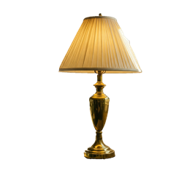
\includegraphics[width=86.25pt,height=72.45pt]{C5PS – DT – Q1i.png}}};
\draw (46,150.2) node [anchor=north west][inner sep=0.75pt]   [align=left] {Lamp};
\end{tikzpicture}
},
optionB={
\tikzset{every picture/.style={line width=0.75pt,scale=\scalefactor}} 
\begin{tikzpicture}[x=0.75pt,y=0.75pt,yscale=-1,xscale=1]
\draw (84.5,96.3) node  {\adjustbox{scale=\scalefactor}{
\includegraphics[width=58.75pt,height=75.45pt]{C5PS – DT – Q1ii.png}}};
\draw (39,152) node [anchor=north west][inner sep=0.75pt]   [align=left] {Lighting bees};
\end{tikzpicture}
},
optionC={
\tikzset{every picture/.style={line width=0.75pt,scale=\scalefactor}}     
\begin{tikzpicture}[x=0.75pt,y=0.75pt,yscale=-1,xscale=1]
\draw (87.2,160.3) node  {\adjustbox{scale=\scalefactor}{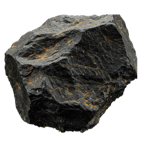
\includegraphics[width=79pt,height=73.95pt]{C5PS – DT – Q1iii.png}}};
\draw (42,213) node [anchor=north west][inner sep=0.75pt]   [align=left] {Rock};
\end{tikzpicture}
},
optionD={
\tikzset{every picture/.style={line width=0.75pt,scale=\scalefactor}} 
\begin{tikzpicture}[x=0.75pt,y=0.75pt,yscale=-1,xscale=1]
\draw (78.2,108.8) node  {\adjustbox{scale=\scalefactor}{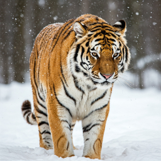
\includegraphics[width=84.9pt,height=74.7pt]{C5PS – DT – Q1iv.png}}};
\draw (34,162) node [anchor=north west][inner sep=0.75pt]   [align=left] {Tiger};
\end{tikzpicture}
},
correctoption={A},
}


\begin{minipage}{\linewidth}
\hspace{1cm}
\centering
\tiny
\renewcommand{\arraystretch}{1.25}
\begin{tabular}{|M{1.2cm}|M{0.8cm}|M{0.8cm}|M{0.8cm}|M{0.8cm}|M{0.8cm}|}
\hline
Option & \cellcolor{cellgreen} A (\ding{51}) & B (\ding{55}) & C (\ding{55}) & D (\ding{55}) & E \\ 
\hline
5 A & \highgreen{82\%} & \highno{0\%} & \highno{18\%} & \highno{0\%} & \highno{0\%} \\ 
 \hline 
5 B & \highgreen{100\%} & \highno{0\%} & \highno{0\%} & \highno{0\%} & \highno{0\%} \\ \hline
\end{tabular}
\end{minipage}

\end{frame}
% \input{4. PPT/My Answer/Science/C5/117_C5S - Q35}


\begin{frame}[shrink=0.1,label=QPC5QC5S10 - DT - Q1]{Q16 [10. Safety and First aid*]}
\vspace{-0.2cm}
\mcqtextbottomFourOne{
  questionnumber={16}, 
  questionTag={C5S10 – DT – Q1}, 
  questiontext={What is the first aid for a minor burn in your hand?},
  optionA={Apply oil as an ointment over the burn area.},
  optionB={Rinse the burn area with cool water.},
  optionC={Apply salt over the burn area.},
  optionD={Cover the burn with plastic paper immediately.},
  correctoption={B},
}

\begin{minipage}{\linewidth}
\hspace{1cm}
\centering
\tiny
\renewcommand{\arraystretch}{1.25}
\begin{tabular}{|M{1.2cm}|M{0.8cm}|M{0.8cm}|M{0.8cm}|M{0.8cm}|M{0.8cm}|}
\hline
Option & A (\ding{55}) & \cellcolor{cellgreen} B (\ding{51}) & C (\ding{55}) & D (\ding{55}) & E \\ 
\hline
5 A & \highno{47\%} & \highno{41\%} & \highno{0\%} & \highno{12\%} & \highno{0\%} \\ 
 \hline 
5 B & \highno{29\%} & \highno{50\%} & \highno{14\%} & \highno{7\%} & \highno{0\%} \\ \hline
\end{tabular}
\end{minipage}

\end{frame}
% \input{4. PPT/My Answer/Science/C5/117_C5S - Q16}

%

    